\Chapter{Die arithmetisch-logische Einheit}
\label{ch:alu}

Die arithmetisch-logische Einheit \textit{ALU} ist verantwortlich f\"ur die Durchf\"uhrung aller f\"ur die Befehlsausf\"uhrung durch das Leitwerk relevanten Rechenoperationen. Zus\"atzlich verwaltet sie die Register des Prozessors.


\Section{\"Uberblick}
Zentrale Design-Idee hinter der ALU ist es, mehr als einen reinen Multiplexer f\"ur Befehle zu entwickeln. Stattdessen bietet sie dem Leitwerk ein Interface,
\"uber das Operationen auf Registern oder Immediates angefragt werden k\"onnen. Hierzu wurde eine Menge von Prozessor-internen Opcodes definiert.

Da die ALU auch zur Ausf\"uhrung von nicht-arithmetischen Maschinenbefehlen, beispielsweise bei Spr\"ungen, oft beansprucht wird, sollte der Synchronisations- und Kommunikationsaufwand zwischen ALU und Leitwerk m\"oglichst reduziert werden.
Aus diesem Grund werden grunds\"atzlich alle Befehle (exklusive der Division) mittels einer Zustandsmaschine innerhalb von drei Takten ausgef\"uhrt, wodurch kein Synchronisations-Protokoll zwischen ALU und Leitwerk von N\"oten ist.

Um die Komplexit\"at des Leitwerks zu reduzieren, wurde die Low-Level-Verwaltung der Register in die ALU ausgelagert. Diese wurden als Dual-Port-Blockram realisiert, um die Anzahl an belegten Slices auf dem FPGA zu reduzieren.

\Section{Das Interface}
\begin{figure}[H]
	\centering
	\label{fig:aluinterface}
		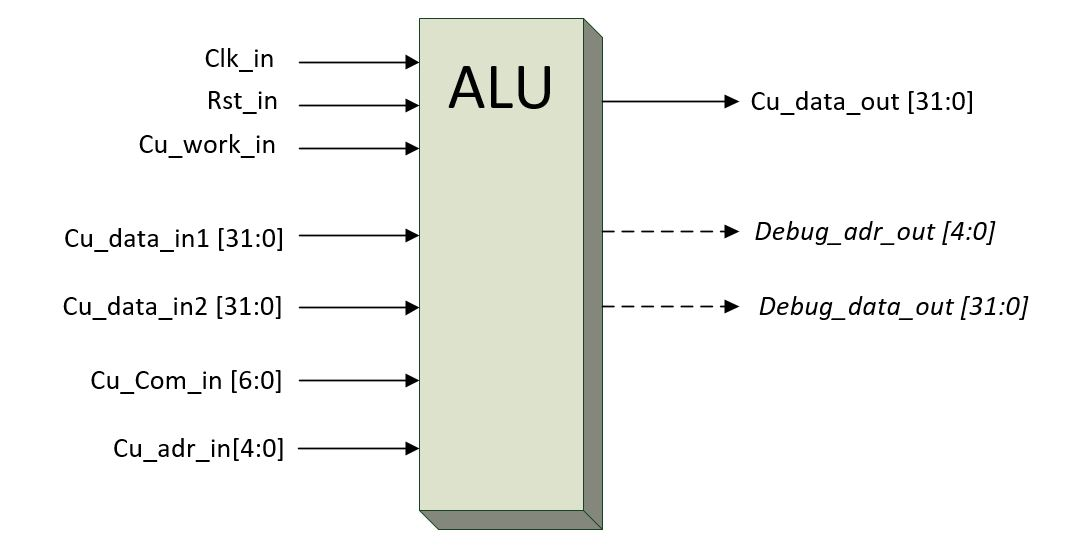
\includegraphics[width=0.7\textwidth]{interface.jpg}
	\caption[Schnittstelle der ALU-Einheit]{Schnittstelle der ALU mit Portnamen und -breiten}
\end{figure}

Neben zwei 32-Bit-Eing\"angen f\"ur Operanden, gibt es einen dedizierten Eingang f\"ur Registeradressen sowie einen zur Auswahl der gew\"unschten Operation. 
Der Adresseingang dient hierbei lediglich zur Adressierung des Zielregisters. Da alle Befehle nur aus zwei Operanden bestehen, werden die Operanden-Eing\"ange entweder zur \"Ubermittlung von Immediates, oder zur Adressierung der Operanden-Register verwendet, was die Anzahl der Eing\"ange reduziert.

Aktiviert wird die ALU vom Leitwerk \"uber \Vhdl{cu\_work\_in}; innerhalb von drei Takten liegt dann auf \Vhdl{cu\_data\_out} das entsprechende Ergebnis an.

\Section{Interne Befehle}
Zur Auswahl der gew\"unschten Operation bietet die ALU einen 7 Bit breiten Befehls-Eingang an.
Jeder Befehl besteht dabei aus drei Sektionen\vspace{10pt}:

\Instr{Reg1 | Reg2 | OpC}\vspace{5pt}

Das oberste Bit \Ipart{Reg1} entscheidet dar\"uber, ob der erste Operand als Immediate vom Dateneingang \Vhdl{cu\_data\_in1}, oder aus dem durch \Vhdl{cu\_data\_in1} adressierten Register genommen wird.
Analog wird anhand \Ipart{Reg2} determiniert, ob auf \Vhdl{cu\_data\_in2} eine Adresse oder ein Immediate anliegt.
Darauf folgt der f\"unf Bit umfassende interne OpCode. Zur Verf\"ugung stehen OpCodes f\"ur:

\begin{itemize}
\item Addition, Subtraktion
\item Logische Shifts
\item Arithmetische Shifts
\item Set Less Than Immediate Signed und Unsigned (SLT,SLTU)
\item Multiply Lower auf Signed und Unsigned-Operanden
\item Multiply Upper auf Signed und Unsigned Operanden
\item Division Signed und Unsigned
\item Modulo-Rechnung Signed und Unsigned
\end{itemize}

\Section{Befehlsausf\"uhrung}


\Statemachine{./alu/img/states.pdf}{
Zustands\"ubergangsdiagramm der Befehlsausf\"uhrung innerhalb der ALU
}{}

Die Ausf\"uhrung von Befehlen ist \"uber eine State-Machine mit drei zentralen Zust\"anden, sowie zwei Zusatzzust\"anden f\"ur Signed- und Unsigned-Division bzw. Modulo-Operationen realisiert. In jedem der drei zentralen Zust\"ande wird dabei nur f\"ur einen Takt verblieben.


\Subsection{State 1 - Selektion der Operanden}
Die ALU wartet in State 1, bis vom Leitwerk das entsprechende Work-Signal gesendet wird.
Anschlie\ss{}end werden auf Grundlage des oben beschriebenen Befehls zwei Operanden-Signale \Vhdl{s\_op1} und \Vhdl{s\_op2} mit einer Immediate vom Daten-Eingang belegt, oder aber es wird ein Register-Lesezugriff angesto"sen, dessen Ergebnis dann im n\"achsten Takt zur Verf\"ugung steht.


\Subsection{State 2 - Operationsausf\"uhrung}
State 2 dient der eigentlichen Befehlsausf\"uhrung. Realisiert ist er als Case-Statement \"uber den internen OpCode. Innerhalb jedes Cases wird zwischen den vier m\"oglichen Kombinationen auf Immediate- und Register-Operanden unterschieden.
Dies ist n\"otig, da das Ergebnis eines m\"oglichen Register-Zugriffs erst in diesem Takt anliegt und deshalb nicht einfach die \Vhdl{s\_op1}- und \Vhdl{s\_op2}-Signale f\"ur Immediate-Operationen \"uberschrieben werden k\"onnen.
Die Operation wird auf den jeweiligen Operanden durchgef\"uhrt und in einem Akkumulator gespeichert.\vspace{10pt}


Ein Gro"steil der Operationen ist \"uber die \Vhdl{IEEE.NUMERIC\_STD.ALL} Operatoren realisiert und kann innerhalb dieses einen Taktes vollst\"andig abgeschlossen werden.

Da die Standard-Multiplikation von 32-Bit-Werten zu einem 64 Bit langen Ergebnis f\"uhrt, werden Multiplikationsergebnisse nicht im normalen Akkumulator-Signal \Vhdl{acc}, sondern im Zusatzsignal \Vhdl{mult-result} gespeichert. Der VHDL-Compiler erlaubte es nicht, unmittelbar auf das Ergebnis zuzugreifen und entweder die oberen oder unteren 32 Bit in \Vhdl{acc} zu speichern.\vspace{10pt}

Da der Standard-Operator \Vhdl{sar} nicht durch die gegebene Entwicklungsumgebung synthetisierbar ist, wird bei einem arithmetischen Rechtsshift um {n} Stellen zus\"atzlich das oberste Bit des ersten Operanden zwischengespeichert, um im nachfolgenden State, wenn n\"otig, die oberen {n} Bits auf {1} zu setzen.\vspace{10pt}

Im Falle einer Modulo- oder Unsigned-Division wird in State 2 der \"Ubergang in State 4 bzw. 5 eingeleitet. Ansonsten erfolgt ein direkter \"Ubergang in State 3.

\Subsection{State 3 - Write-Back}
In State 3 werden die akkumulierten Ergebnisse in das von der ALU adressierte Register geschrieben.

Bei den meisten der Operationen kann dies unmittelbar erfolgen. Bei Multiplikationsoperationen allerdings muss jedoch zuerst anhand des OpCodes entschieden werden, ob die oberen oder unteren 32 Bit des Ergebnisses gespeichert werden sollen. Abh\"angig vom Status-Bit f\"ur arithmetische Shifts um {n} Stellen werden, wie oben beschrieben, gegebenenfalls die oberen n Bits des Ergebnisses auf {1} gesetzt.\vspace{10pt}


Neben dem Speichern des Ergebnisses werden zwei zus\"atzliche Ausg\"ange belegt:

Auf \Vhdl{cu\_data\_out} wird das Ergebnis angelegt. Einzige Ausnahme stellt die Division bzw. Modulorechnung dar, bei der als Synchronisationssignal der Daten-Ausgang mit 0 belegt wird. Das ist n\"otig, da die Division vom normalen 3-Takte-Schema abweicht.
Auch die Debug-Schnittstelle erh\"alt \"uber \Vhdl{debug\_data\_out} den entsprechenden Wert sowie das relevante Register \"uber \Vhdl{debug\_adr\_out}.

\Subsection{State 4 - Division Unsigned}
Um die Anzahl an n\"otigen Takten zu reduzieren, wird bei der Umsetzung der Unsigned Division eine durch den \textit{Core-Generator} erstellte Divisionseinheit genutzt, welche eine gepipelinte Variante der SRT-Division durchf\"uhrt. Obwohl der Prozessor keinen unmittelbaren Nutzen aus dem Pipelining zieht, kann durch die effiziente Implementierung die Anzahl an n\"otigen Takten reduziert werden. Zus\"atzlich liefert die Einheit sowohl den Rest, als auch das Divisionsergebnis, weshalb die beiden Operationen gleich behandelt werden k\"onnen.


Hierzu werden bei Betreten des States die Operanden angelegt. Danach wird mit einem Z\"ahler gewartet, bis das Ergebnis der Operation anliegt.
Anschlie\ss{}end werden je nach Anfrage entweder der Rest oder das Ergebnis in den Akkumulator eingelesen und in State 3 \"ubergegangen.

\Subsection{State 5 - Division Signed}
Die Implementierung verl\"auft analog zu State 4, abgesehen davon, dass eine Einheit zur Durchf\"uhrung von Signed-Divisionen verwendet wird.

\Section{Die Register}
Insgesamt stellt die ALU 32 Register der Breite 32 Bit bereit, wobei Register x0 konstant mit dem Wert 0 belegt und nicht \"uberschreibbar ist. Dies ist zum Beispiel n\"utzlich beim unver\"anderten Laden eines Registers.

Implementiert wurden die Register als Dual-Port-Blockram. Dieses Vorgehen erm\"oglicht den zeitgleichen Zugriff auf zwei verschiedene Speicherinhalte, was gerade bei Register-Register-Operationen von Vorteil ist. Zus\"atzlich wird dadurch die Anzahl an verwendeten Slices reduziert, da dedizierte Blockram-Bausteine logisch zum Registersatz zusammengef\"ugt werden.\vspace{10pt}

Die Umsetzung erfolgte dabei nicht \"uber eine Variante aus dem \textit{Core-Generator}, sondern durch die Einhaltung eines speziellen Verwendungsprotokolls, sodass der Compiler das definierte \textit{std\_logic\_vector}-Array automatisch in einen Blockram umsetzt.

Voraussetzung daf\"ur ist, dass nicht direkt auf Register-Inhalten operiert wird, sondern sie zuerst in einem Signal zwischengespeichert und im n\"achsten Takt verwendet werden. Dies ist aber ohnehin durch die 3-stufige State-Machine der ALU garantiert.

\Section{Reset}
Die ALU verf\"ugt zudem \"uber einen Reset-Eingang, welcher direkt von der Toplevel-Komponente weitergeleitet wird. Bei einem Reset wird das Rechenwerk in den State 0 \"uberf\"uhrt, um nach Ende des Resets wieder Befehle des Leitwerks entgegennehmen zu k\"onnen.

Zus\"atzlich wird der Divisions-Flankenz\"ahler auf Null gesetzt, um keine Fehler bei nachfolgenden Operationen zu versursachen. Das Reset-Signal wird auch an den Reset (SCLR)-Eingang der Divisionseinheit weitergeleitet.

Ein Reset der Register erfolgt nicht, sodass abgesehen vom Register x0 f\"ur den Entwickler eines Nutzerprogramms keine Aussage \"uber die initialen Werte der Register m\"oglich ist.

\newpage
